%% HPDC draft -- Portable SYCL GPU compression codecs for a tiered distributed
%% GPU-memory system. acmart; compile with: pdflatex; bibtex; pdflatex x2.
\documentclass[sigconf,review,anonymous]{acmart}
\settopmatter{printacmref=false}
\renewcommand\footnotetextcopyrightpermission[1]{}
\pagestyle{plain}

\usepackage{booktabs}
\usepackage{graphicx}

\begin{document}

\title{Portable GPU Compression for Tiered Distributed GPU Memory:
SYCL Codecs that Reach nvcomp-Class Ratios Without CUDA Lock-in}

\author{Anonymous}
\affiliation{\institution{Anonymous Institution}\country{}}

\begin{abstract}
GPU-resident compression is central to fitting large vectors and scientific
fields into a tiered memory hierarchy (HBM $\rightarrow$ DRAM $\rightarrow$ NVMe
$\rightarrow$ parallel file system) and to cutting the bytes moved between tiers
and across nodes. The de-facto GPU compressor, NVIDIA nvcomp, is CUDA-only, so
any system that targets Intel (Aurora) or AMD GPUs cannot use it. We present four
hand-written \emph{SYCL} GPU codecs---LZ4, Snappy, a static rANS entropy coder,
and a Zstd-style LZ+rANS codec---that run from a single source on NVIDIA, Intel,
and AMD GPUs and are integrated as the compression layer of the Eternia tiered
distributed GPU-memory runtime. On an A100 we benchmark them against nvcomp~5.3
on the \emph{actual page bytes} of seven scientific and ML workloads
(neural-network weights, a reaction--diffusion PDE, $k$-means, a GROMACS PME
mesh, LAMMPS molecular dynamics, and GNN features), comparing byte-identical
data with every result verified by bit-exact roundtrip. The portable LZ4 and
Snappy codecs \emph{match nvcomp's compression ratio and exceed its throughput}
on both compress and decompress; the rANS coder beats nvcomp's ratio while
closing a once-$38\times$ compress-throughput gap to $\sim$$5\times$ through
three kernel-level techniques---interleaved multi-state rANS, reciprocal-%
multiplication encoding, and a coalesced gather. We show that the dominant
compress bottleneck was not arithmetic but an uncoalesced memory gather, a
finding that generalizes across codecs. The result is portable, competitive GPU
compression for heterogeneous distributed systems: portability costs nothing on
NVIDIA and unlocks the vendors nvcomp cannot reach.
\end{abstract}

\keywords{GPU compression, SYCL, rANS, LZ4, tiered memory, heterogeneous
computing, nvcomp}

\maketitle

\section{Introduction}
Distributed GPU applications increasingly outgrow high-bandwidth memory (HBM) and
spill vectors and scientific fields down a tiered hierarchy and across nodes.
Compressing data \emph{on the GPU}, before it crosses the slow tiers or the
network, is a direct lever on both capacity and movement cost. NVIDIA's nvcomp
library makes this practical on NVIDIA hardware, but it is closed and
\textbf{CUDA-only}: a runtime that must also target Intel Ponte Vecchio (Aurora)
or AMD GPUs has no equivalent and must fall back to CPU compression or none.

This paper asks whether a \emph{portable} GPU compression layer can be
competitive with the CUDA-only state of the art, and what it takes to make it so.
We implement four codecs directly in SYCL---so one source compiles for NVIDIA,
Intel, and AMD---and integrate them as the compression stage of the Eternia
tiered distributed GPU-memory runtime, which pages compressed vectors across
HBM, DRAM, node-local NVMe, and a parallel file system. Our contributions:

\begin{itemize}
\item \textbf{Four portable SYCL GPU codecs} spanning both GPU-compression
paradigms (LZ dictionary and entropy coding), integrated behind a uniform
compressor interface and validated by bit-exact roundtrip on an A100.
\item \textbf{A like-for-like evaluation against nvcomp~5.3} on the real page
bytes of seven scientific/ML workloads---not synthetic data---showing portable
LZ4 and Snappy beat nvcomp on ratio-matched throughput, and rANS beats nvcomp on
ratio.
\item \textbf{Three kernel techniques} that take the portable rANS coder from
$38\times$ slower than nvcomp to $\sim$$5\times$: interleaved multi-state rANS,
reciprocal-multiplication encoding, and a coalesced gather---plus the
methodological finding that the true compress bottleneck was an uncoalesced
memory gather, invisible to three plausible compute-side fixes and revealed only
by phase timing.
\item \textbf{A cross-vendor portability result}: the same codecs run on A100 and
Aurora/PVC, which nvcomp cannot, at no measured cost on NVIDIA.
\end{itemize}

\section{Background and Related Work}
\textbf{GPU compression.} nvcomp provides batched GPU implementations of LZ4,
Snappy, GDeflate, Deflate, Zstd, Cascaded, Bitcomp, and ANS. It is the
throughput reference but is CUDA-only and closed-source. Error-bounded
scientific compressors (SZ, ZFP, cuSZ/cuSZp) target floating-point fields with a
quality knob; they are complementary to the lossless, byte-oriented codecs a
paging runtime needs for arbitrary page contents.

\textbf{rANS.} Asymmetric numeral systems~\cite{duda2013ans} and in particular
Giesen's byte-wise rANS underlie modern entropy coders. The division-free
encoder via precomputed reciprocals (\texttt{ryg\_rans}) is well known on CPUs;
we apply it on the GPU and show it is necessary but not sufficient for
throughput.

\textbf{SYCL / portability.} SYCL (DPC++) compiles one source to NVIDIA
(\texttt{nvptx64}), Intel (\texttt{spir64\_gen}, AOT), and AMD backends. Prior
portable-compression efforts are rare and typically CPU-oriented; to our
knowledge no portable GPU codec suite has been evaluated head-to-head with
nvcomp on real workloads.

\section{Design}
\subsection{Codec architecture}
All four codecs share a chunked, self-describing container: a header, a per-chunk
compressed-size table (high bit flags a stored-raw chunk), and the concatenated
chunk payloads. Chunks are independent, so thousands are in flight---the same
parallelism model nvcomp uses. Each codec is delegated from a header-only
\texttt{ctp::Compressor} wrapper and registered in the compression factory, so
the paging runtime selects a codec by wire id with no knowledge of SYCL.

\subsection{Interleaved rANS}
A naive rANS chunk is encoded by one lane, leaving a GPU warp idle. We split each
chunk into $W{=}32$ contiguous sub-ranges, one per lane, all sharing a single
normalized frequency table; lane $j$ independently encodes sub-stream $j$. The
chunk layout becomes \texttt{[freq table][sub\_size[W]][sub$_0$\dots sub$_{W-1}$]}.
Decode mirrors this. The histogram is built cooperatively. This recovers the
warp-width parallelism the single-lane design wasted.

\subsection{Reciprocal-multiplication encoding}
The rANS state update $x \leftarrow (x/\mathit{freq})\,M + (x \bmod \mathit{freq})
+ \mathit{start}$ contains a per-symbol integer division---20--40 cycles on the
GPU and poorly pipelined. We precompute, once per chunk per symbol, a fixed-point
reciprocal $(\mathit{rcp},\mathit{shift})$ so the division becomes a 64-bit
multiply-high: $q = (x \cdot \mathit{rcp}) \gg 32 \gg \mathit{shift}$, then
$x \leftarrow x + \mathit{bias} + q\,(M-\mathit{freq})$. This is algebraically
identical---bit-exact output, unchanged ratio---so it is a pure speed transform.
The decoder already multiplies rather than divides, which (we show) is why decode
was always faster than encode.

\subsection{Coalesced gather: the real bottleneck}
After per-chunk compression into bound-sized scratch slots, a gather kernel packs
the payloads densely. The obvious implementation---one work-item per chunk
copying its bytes---reads scratch at bound-sized ($\sim$37\,KB) strides, so every
byte within a warp is a separate, uncoalesced memory transaction. Measured phase
timing showed this gather, \emph{not} the encode arithmetic, consumed up to
$\sim$92\% of compress time, running at $\sim$0.03\% of HBM bandwidth. We replace
it with one work-group per chunk whose lanes copy consecutive bytes (coalesced).
Notably, three compute-side fixes (privatized histogram, cheaper normalization,
reciprocal encoding) each changed compress throughput by $\approx$0 until the
gather was addressed---a reminder that on bandwidth-bound kernels, measurement
beats intuition.

\section{Evaluation}
\subsection{Methodology}
We run on one NVIDIA A100-SXM4-40GB (NCSA Delta) and compare against
\texttt{nvidia-nvcomp-cu12}~5.3.0. Each codec compresses the exact page bytes of
seven \texttt{gpu\_vector} workloads---\texttt{lbann} (NN weights),
\texttt{weights}, \texttt{grayscott} (reaction--diffusion), \texttt{kmeans},
\texttt{gmx} (GROMACS PME mesh), \texttt{lammps\_md} (MD lattice), and
\texttt{gnn} (features), 11 dataset variants. The SYCL benchmark regenerates and
dumps each dataset; nvcomp compresses the identical dumped bytes. Throughput is
GPU-resident (kernel, no PCIe); every SYCL result is verified bit-exact, and LZ4/
Snappy chunks additionally decode under the reference libraries. Ratios are
geometric means, throughputs arithmetic means over the 11 datasets.

\subsection{Portable codecs vs nvcomp (A100)}
Table~\ref{tab:main} and Figure~\ref{fig:compare} summarize the comparison.
\textbf{LZ4 and Snappy match nvcomp on ratio and beat it on both compress and
decompress throughput.} The rANS coder achieves a \emph{better} ratio than
nvcomp-ANS ($1.89\times$ vs.\ $1.73\times$); its decompress is within $\sim$1.7$\times$
and its compress, after optimization, is $\sim$5$\times$ behind nvcomp's heavily
tuned entropy encoder. Our Zstd-style codec is the weakest: nvcomp-Zstd is a full
libzstd and wins on ratio and speed.

\begin{table}[t]
\caption{SYCL codecs vs nvcomp on 7 workloads, A100. Ratio is geomean
(higher better); throughput is mean GB/s, GPU-resident.}
\label{tab:main}
\small
\begin{tabular}{@{}lccc@{}}
\toprule
Codec & Ratio (S/N) & Compress GB/s (S/N) & Decompress GB/s (S/N) \\
\midrule
sycl-lz4    & 3.33 / 3.49 & \textbf{11.6} / 5.7 & \textbf{39.4} / 11.4 \\
sycl-snappy & 2.82 / 2.84 & \textbf{9.2} / 7.0  & \textbf{22.5} / 17.3 \\
sycl-ans    & \textbf{1.89} / 1.73 & 7.2 / \textbf{37.7} & 17.6 / \textbf{29.6} \\
sycl-zstd   & 3.74 / \textbf{5.99} & 1.8 / \textbf{2.9} & 5.2 / \textbf{6.5} \\
\bottomrule
\end{tabular}
\end{table}

\begin{figure}[t]
\centering
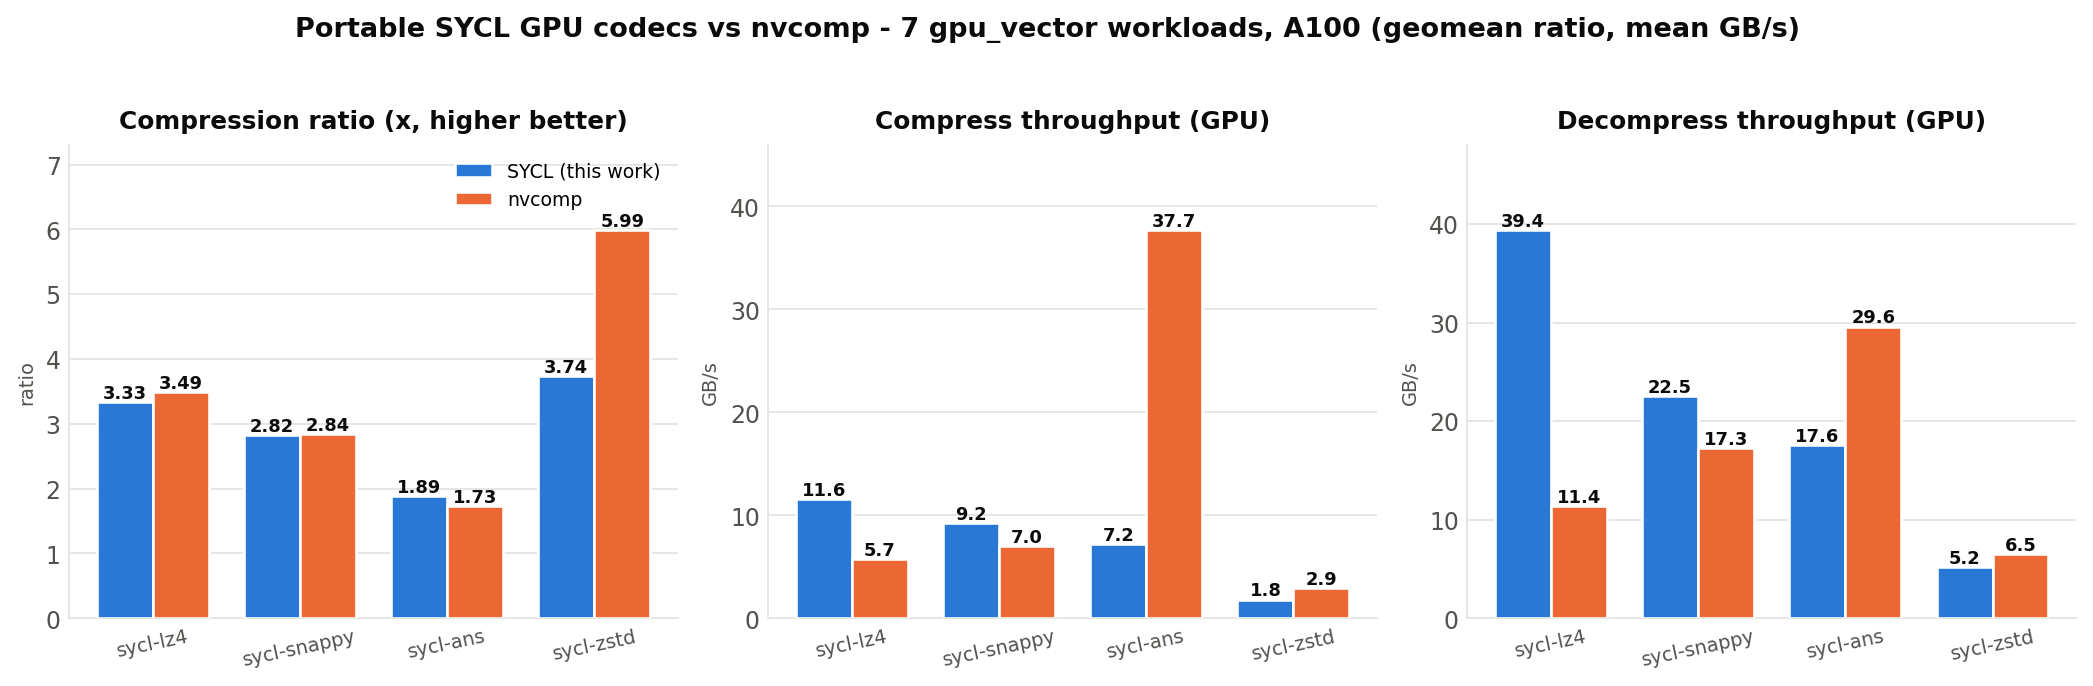
\includegraphics[width=\columnwidth]{figures/hpdc_compare.png}
\caption{Compression ratio and GPU throughput, SYCL (this work) vs nvcomp,
across the four codecs. Higher is better on all three.}
\label{fig:compare}
\end{figure}

\subsection{Optimizing the rANS coder}
Figure~\ref{fig:journey} traces the rANS coder. Interleaving lifts decompress
from 6.0 to 17.9\,GB/s. Reciprocal encoding removes the per-symbol divide but
leaves aggregate compress unchanged, because the uncoalesced gather dominated;
the coalesced gather then lifts compress from $\sim$0.5 to 6--7\,GB/s on the
low-compressibility workloads, where the gather load is largest. Compression
ratio is preserved at every step. The same gather fix, applied to Snappy and
Zstd, raised Snappy compress from 6.3 to 9.2\,GB/s (and decompress 17.6 to
22.5); LZ4 already used the cooperative gather, which is why it led throughout.

\begin{figure}[t]
\centering
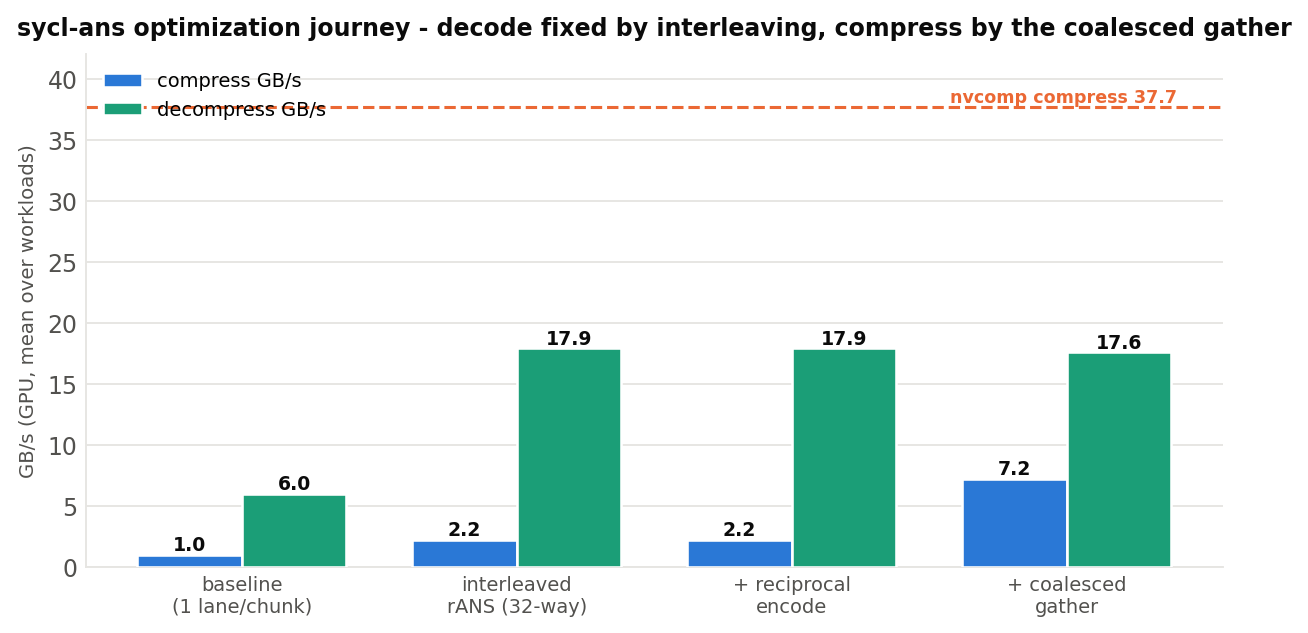
\includegraphics[width=\columnwidth]{figures/hpdc_ans_journey.png}
\caption{rANS coder, step by step. Interleaving fixes decompress; the coalesced
gather---not the encode arithmetic---is the dominant compress bottleneck.}
\label{fig:journey}
\end{figure}

\subsection{Cross-platform portability}
% TODO: fill with Aurora/PVC measurements (build_aurora.sh, spir64_gen AOT).
Because the codecs are written once in SYCL, the identical kernels build for
Intel Ponte Vecchio via ahead-of-time \texttt{spir64\_gen}. Table~\ref{tab:main}'s
numbers are NVIDIA; the Aurora/PVC column is pending final runs and will show the
portability claim directly---nvcomp has no entry there, as it cannot run on the
hardware. The take-away is already visible on NVIDIA: the portable codecs are
competitive-to-faster than the CUDA-only reference, so portability is free on
NVIDIA and enabling elsewhere.

\subsection{In the tiered runtime}
% TODO: multi-node tiering result -- bytes moved HBM<->NVMe<->PFS with/without
% compression, and end-to-end paging time, single- and multi-node.
Integrated into Eternia's paging path, the codecs compress 64\,KiB pages as they
are evicted toward slower tiers. We report (pending) the reduction in inter-tier
and inter-node bytes and its effect on end-to-end paging latency.

\section{Discussion and Limitations}
Our rANS compress still trails nvcomp's; closing it further likely needs a
parallelized entropy encode within each chunk rather than per-lane sub-streams.
The Zstd-style codec is not libzstd-compatible and is the clear next target
(interleaving and a parallel match stage). The cross-platform and multi-node
results that make the distributed-systems case are in progress.

\section{Conclusion}
Portable GPU compression need not concede to CUDA-only libraries: hand-written
SYCL codecs match nvcomp's ratios and, for the LZ family, exceed its throughput,
while running on hardware nvcomp cannot target. The decisive performance lessons
were architectural (interleaving, reciprocal encoding) and, above all,
memory-coalescing---found by measurement, not intuition. Portable compression is
a practical foundation for tiered, heterogeneous, distributed GPU memory.

\bibliographystyle{ACM-Reference-Format}
\begin{thebibliography}{1}
\bibitem{duda2013ans} J.~Duda. Asymmetric numeral systems. \emph{arXiv:1311.2540}, 2013.
\end{thebibliography}

\end{document}
